
%%--------------------------------------------------
%% Halliday: Fundamentals of Physics
%%--------------------------------------------------


%% Chapter 13: Gravitation
%%--------------------------------------------------


%% Learning Objectives
%%--------------------------------------------------

%% 13.01: Apply Newton's law of gravitation to relate the gravitational force between two particles to their masses and their separation.
%% 13.02: Identify that a uniform spherical shell of matter attracts a particle that is outside the shell as if all the shell's mass were concentrated as a particle at its center.
%% 13.03: Draw a free-body diagram to indicate the gravitational force on a particle due to another particle or a uniform, spherical distribution of matter.


%% Halliday Multiple Choice Questions
%%--------------------------------------------------
\element{halliday-mc}{
\begin{question}{halliday-ch13-q01}
    In the formula $F = Gm_1 m_2/r^2$, the quantity $G$:
    \begin{choices}
        \wrongchoice{depends on the local value of g}
        \wrongchoice{is used only when Earth is one of the two masses}
        \wrongchoice{is greatest at the surface of Earth}
      \correctchoice{is a universal constant of nature}
        \wrongchoice{is related to the Sun in the same way that g is related to Earth}
    \end{choices}
\end{question}
}

\element{halliday-mc}{
\begin{question}{halliday-ch13-q02}
    The magnitude of the acceleration of a planet in orbit around the Sun is proportional to:
    \begin{choices}
        \wrongchoice{the mass of the planet}
      \correctchoice{the mass of the Sun}
        \wrongchoice{the distance between the planet and the Sun}
        \wrongchoice{the reciprocal of the distance between the planet and the Sun}
        \wrongchoice{the product of the mass of the planet and the mass of the Sun}
    \end{choices}
\end{question}
}

\element{halliday-mc}{
\begin{question}{halliday-ch13-q03}
    Suitable units for the gravitational constant $G$ are:
    \begin{choices}
        \wrongchoice{kilogram meter per second squared (\si{\kilo\gram\meter\per\second\squared})}
        \wrongchoice{meter per second squared (\si{\meter\per\second\squared})}
        \wrongchoice{newton second per meter (\si{\newton\second\per\meter})}
        \wrongchoice{kilogram meter per second (\si{\kilo\gram\meter\per\second})}
      \correctchoice{meter cubed per kilogram per second squared (\si{\meter\cubed\per\kilo\gram\per\second\squared})}
    \end{choices}
\end{question}
}

\element{halliday-mc}{
\begin{question}{halliday-ch13-q04}
    The gravitational constant $G$ has the derived units:
    \begin{choices}
        \wrongchoice{newton meter (\si{\newton\meter})}
        \wrongchoice{newton meter per kilogram (\si{\newton\meter\per\kilo\gram})}
        \wrongchoice{newton kilogram  per meter (\si{\newton\kilo\gram\per\meter})}
      \correctchoice{newton meter squared per kilogram squared (\si{\newton\meter\squared\per\kilo\gram\squared})}
        \wrongchoice{newton kilogram squared per meter squared (\si{\newton\kilo\gram\squared\per\meter\squared})}
    \end{choices}
\end{question}
}

\element{halliday-mc}{
\begin{question}{halliday-ch13-q05}
    Earth exerts a gravitational force on the Moon,
        keeping it in its orbit. 
    The reaction to this force, in the sense of Newton's third law, is:
    \begin{choices}
        \wrongchoice{the centripetal force on the Moon}
        \wrongchoice{the nearly circular orbit of the Moon}
      \correctchoice{the gravitational force on Earth by the Moon}
        \wrongchoice{the tides due to the Moon}
        \wrongchoice{the apple hitting Newton on the head.}
    \end{choices}
\end{question}
}

\element{halliday-mc}{
\begin{question}{halliday-ch13-q06}
    A particle might be placed
    \begin{enumerate}
        \item inside a uniform spherical shell of mass $M$, but not at the center
        \item inside a uniform spherical shell of mass $M$, at the center
        \item outside a uniform spherical shell of mass $M$, a distance $r$ from the center
        \item outside a uniform solid sphere of mass $M$, a distance $2r$ from the center
    \end{enumerate}
    Rank these situations according to the magnitude of the gravitational
        force on the particle, least to greatest.
    \begin{choices}
        \wrongchoice{All tie}
        \wrongchoice{1, 2, 3, 4}
        \wrongchoice{1 and 2 tie, then 3 and 4 tie}
      \correctchoice{1 and 2 tie, then 3, then 4}
        \wrongchoice{1 and 2 tie, then 4, then 3}
    \end{choices}
\end{question}
}

\element{halliday-mc}{
\begin{question}{halliday-ch13-q07}
    Three particles, two with mass $m$ and one with mass $M$,
        might be arranged in any of the four configurations known below. 
    Rank the configurations according to the magnitude of the gravitational force on $M$,
        least to greatest.
    \begin{center}
    \hfill
    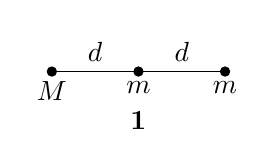
\begin{tikzpicture}[scale=1.1]
        \draw[white] (-1.2,-0.3) rectangle (1.2,0.5);
        \draw[fill] (-1,0) circle (1.5pt) node[anchor=north] {$M$};
        \draw[fill] (+0,0) circle (1.5pt) node[anchor=north] {$m$};
        \draw[fill] (+1,0) circle (1.5pt) node[anchor=north] {$m$};
        \draw (-1,0) -- (0,0) node[pos=0.5,anchor=south] {$d$};
        \draw (+1,0) -- (0,0) node[pos=0.5,anchor=south] {$d$};
        \node[anchor=north] at (0,-1em) {\bfseries 1};
    \end{tikzpicture}
    \hfill
    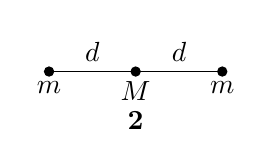
\begin{tikzpicture}[scale=1.1]
        \draw[white] (-1.2,-0.3) rectangle (1.2,0.5);
        \draw[fill] (-1,0) circle (1.5pt) node[anchor=north] {$m$};
        \draw[fill] (+0,0) circle (1.5pt) node[anchor=north] {$M$};
        \draw[fill] (+1,0) circle (1.5pt) node[anchor=north] {$m$};
        \draw (-1,0) -- (0,0) node[pos=0.5,anchor=south] {$d$};
        \draw (+1,0) -- (0,0) node[pos=0.5,anchor=south] {$d$};
        \node[anchor=north] at (0,-1em) {\bfseries 2};
    \end{tikzpicture}
    \hfill~ \\[\baselineskip]
    \hfill
    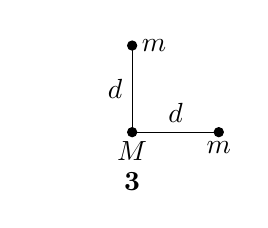
\begin{tikzpicture}[scale=1.1]
        \draw[white] (-1.2,-0.3) rectangle (1.2,1.2);
        \draw[fill] (0,1) circle (1.5pt) node[anchor=west] {$m$};
        \draw[fill] (+0,0) circle (1.5pt) node[anchor=north] {$M$};
        \draw[fill] (+1,0) circle (1.5pt) node[anchor=north] {$m$};
        \draw (0,1) -- (0,0) node[pos=0.5,anchor=east] {$d$};
        \draw (+1,0) -- (0,0) node[pos=0.5,anchor=south] {$d$};
        \node[anchor=north] at (0,-1em) {\bfseries 3};
    \end{tikzpicture}
    \hfill
    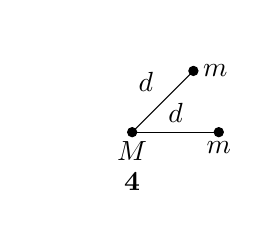
\begin{tikzpicture}[scale=1.1]
        \draw[white] (-1.2,-0.3) rectangle (1.2,1.2);
        \draw[fill] (45:1) circle (1.5pt) node[anchor=west] {$m$};
        \draw[fill] (+0,0) circle (1.5pt) node[anchor=north] {$M$};
        \draw[fill] (+1,0) circle (1.5pt) node[anchor=north] {$m$};
        \draw (0,0) -- (45:1) node[pos=0.5,anchor=south east] {$d$};
        \draw (0,0) -- (1,0) node[pos=0.5,anchor=south] {$d$};
        \node[anchor=north] at (0,-1em) {\bfseries 4};
    \end{tikzpicture}
    \hfill~
    \end{center}
    \begin{multicols}{2}
    \begin{choices}
        \wrongchoice{1, 2, 3, 4}
      \correctchoice{2, 1, 3, 4}
        \wrongchoice{2, 1, 4, 3}
        \wrongchoice{2, 3, 4, 2}
        \wrongchoice{2, 3, 2, 4}
    \end{choices}
    \end{multicols}
\end{question}
}

\element{halliday-mc}{
\begin{question}{halliday-ch13-q08}
    Four particles, each with mass $m$ are arranged symmetrically about the origin on the $x$ axis.
    A fifth particle, with mass $M$, is on the $y$ axis. 
    The direction of the gravitational force on $M$ is:
    \begin{center}
    \begin{tikzpicture}
        \draw (-3,0) -- (3,0);
        \draw (0,0) -- (0,3) node[anchor=north east] {$y$};
        \draw[fill] (0,2) circle (1.5pt) node[anchor=west] {$M$};
        \draw[fill] (-1,0) circle (1.5pt) node[anchor=north] {$m$};
        \draw[fill] (-2,0) circle (1.5pt) node[anchor=north] {$m$};
        \draw[fill] (+1,0) circle (1.5pt) node[anchor=north] {$m$};
        \draw[fill] (+2,0) circle (1.5pt) node[anchor=north] {$m$};
    \end{tikzpicture}
    \end{center}
    \begin{multicols}{3}
    \begin{choices}
        \AMCboxDimensions{down=-0.4cm}
        \wrongchoice{
            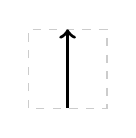
\begin{tikzpicture}
                \draw[dashed,white!80!black] (0,0) rectangle (1,1);
                \draw[very thick,->] (0.5,0) -- (0.5,1);
            \end{tikzpicture}
        }
        %% ANS is B
        \correctchoice{
            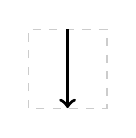
\begin{tikzpicture}
                \draw[dashed,white!80!black] (0,0) rectangle (1,1);
                \draw[very thick,->] (0.5,1) -- (0.5,0);
            \end{tikzpicture}
        }
        \wrongchoice{
            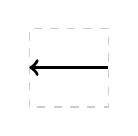
\begin{tikzpicture}
                \draw[dashed,white!80!black] (0,0) rectangle (1,1);
                \draw[very thick,->] (1,0.5) -- (0,0.5);
            \end{tikzpicture}
        }
        \wrongchoice{
            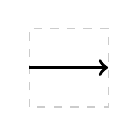
\begin{tikzpicture}
                \draw[dashed,white!80!black] (0,0) rectangle (1,1);
                \draw[very thick,->] (0,0.5) -- (1,0.5);
            \end{tikzpicture}
        }
        \wrongchoice{
            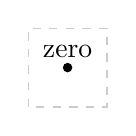
\begin{tikzpicture}
                \draw[dashed,white!80!black] (0,0) rectangle (1,1);
                \draw[fill] (0.5,0.5) circle (1.5pt) node[anchor=south] {zero};
                %\node[anchor=center,text width=10em,text centered] at (0.5,0.5) {none of the provided};
            \end{tikzpicture}
        }
    \end{choices}
    \end{multicols}
\end{question}
}

\element{halliday-mc}{
\begin{question}{halliday-ch13-q09}
    Let $F_1$ be the magnitude of the gravitational force exerted on the Sun by Earth and $F_2$ be the magnitude of the force exerted on Earth by the Sun. 
    Then:
    \begin{choices}
        \wrongchoice{$F_1$ is much greater than $F_2$}
        \wrongchoice{$F_1$ is slightly greater than $F_2$}
      \correctchoice{$F_1$ is equal to $F_2$}
        \wrongchoice{$F_1$ is slightly less than $F_2$}
        \wrongchoice{$F_1$ is much less than $F_2$}
    \end{choices}
\end{question}
}

\element{halliday-mc}{
\begin{question}{halliday-ch13-q10}
    Let $M$ denote the mass of Earth and let $R$ denote its radius. 
    The ratio $g/G$ at Earth's surface is:
    \begin{multicols}{3}
    \begin{choices}
        \wrongchoice{$\dfrac{R^2}{M}$}
      \correctchoice{$\dfrac{M}{R^2}$}
        \wrongchoice{$M R^2$}
        \wrongchoice{$\dfrac{M}{R}$}
        \wrongchoice{$\dfrac{R}{M}$}
    \end{choices}
    \end{multicols}
\end{question}
}

\element{halliday-mc}{
\begin{question}{halliday-ch13-q11}
    Venus has a mass of about \num{0.0558} times the mass of Earth and a diameter of about \num{0.381} times the diameter of Earth. 
    The acceleration of a body falling near the surface of Venus is about:
    \begin{multicols}{2}
    \begin{choices}
        \wrongchoice{\SI{0.21}{\meter\per\second\squared}}
        \wrongchoice{\SI{1.4}{\meter\per\second\squared}}
        \wrongchoice{\SI{2.8}{\meter\per\second\squared}}
      \correctchoice{\SI{3.8}{\meter\per\second\squared}}
        \wrongchoice{\SI{25}{\meter\per\second\squared}}
    \end{choices}
    \end{multicols}
\end{question}
}

\element{halliday-mc}{
\begin{question}{halliday-ch13-q12}
    The approximate value of $g$ at an altitude above Earth equal to one Earth diameter is:
    \begin{multicols}{2}
    \begin{choices}
        \wrongchoice{\SI{9.8}{\meter\per\second\squared}}
        \wrongchoice{\SI{4.9}{\meter\per\second\squared}}
        \wrongchoice{\SI{2.5}{\meter\per\second\squared}}
        \wrongchoice{\SI{1.9}{\meter\per\second\squared}}
      \correctchoice{\SI{1.1}{\meter\per\second\squared}}
    \end{choices}
    \end{multicols}
\end{question}
}

\element{halliday-mc}{
\begin{question}{halliday-ch13-q13}
    A rocket ship is coasting toward a planet. 
    Its captain wishes to know the value of $g$ at the surface of the planet. 
    This may be inferred by:
    \begin{choices}
        \wrongchoice{measuring the apparent weight of one of the crew}
        \wrongchoice{measuring the apparent weight of an object of known mass in the ship}
        \wrongchoice{measuring the diameter of the planet}
        \wrongchoice{measuring the density of the planet}
        \wrongchoice{observing the ship's acceleration and correcting for the distance from the center of the planet.}
    \end{choices}
\end{question}
}

\element{halliday-mc}{
\begin{question}{halliday-ch13-q14}
    To measure the mass of a planet with the same radius as Earth,
        an astronaut drops an object from rest (relative to the planet) from an altitude of one radius above the surface.
    When the object hits its speed is 4 times what it would be if the same experiment were carried out for Earth.
    In units of Earth masses, the mass of the planet is:
    \begin{multicols}{3}
    \begin{choices}
        \wrongchoice{\num{2}}
        \wrongchoice{\num{4}}
        \wrongchoice{\num{8}}
      \correctchoice{\num{16}}
        \wrongchoice{\num{32}}
    \end{choices}
    \end{multicols}
\end{question}
}

\element{halliday-mc}{
\begin{question}{halliday-ch13-q15}
    Suppose you have a pendulum clock that keeps correct time on Earth (acceleration due to gravity = \SI{9.8}{\meter\per\second\squared}).
    Without changing the clock, you take it to the Moon (acceleration due to gravity = \SI{1.6}{\meter\per\second\squared}). 
    For every hour interval (on Earth) the Moon clock will record:
    \begin{multicols}{3}
    \begin{choices}
        \wrongchoice{$\dfrac{9.8}{1.6}\,\si{\hour}$}
        \wrongchoice{$1.0\,\si{\hour}$}
        \wrongchoice{$\sqrt{\dfrac{9.8}{1.6}}\,\si{\hour}$}
        \wrongchoice{$\dfrac{1.6}{9.8}\,\si{\hour}$}
      \correctchoice{$\sqrt{\dfrac{1.6}{9.8}}\,\si{\hour}$}
    \end{choices}
    \end{multicols}
\end{question}
}

\element{halliday-mc}{
\begin{question}{halliday-ch13-q16}
    The mass of an object:
    \begin{choices}
        \wrongchoice{is slightly different at different locations on Earth}
        \wrongchoice{is a vector}
      \correctchoice{is independent of the acceleration due to gravity}
        \wrongchoice{is the same for all objects of the same size and shape}
        \wrongchoice{can be measured directly and accurately on a spring scale}
    \end{choices}
\end{question}
}

\element{halliday-mc}{
\begin{question}{halliday-ch13-q17}
    An astronaut on the Moon simultaneously drops a feather and a hammer. 
    The fact that they land together shows that:
    \begin{choices}
        \wrongchoice{no gravity forces act on a body in a vacuum}
        \wrongchoice{the acceleration due to gravity on the Moon is less than on Earth}
      \correctchoice{in the absence of air resistance all bodies at a given location fall with the same acceleration}
        \wrongchoice{the feather has a greater weight on the Moon than on Earth}
        \wrongchoice{$G = 0$ on the Moon}
    \end{choices}
\end{question}
}

\element{halliday-mc}{
\begin{question}{halliday-ch13-q18}
    The mass of a hypothetical planet is $1/100$ that of Earth and its radius is $1/4$ that of Earth.
    If a person weighs \SI{600}{\newton} on Earth,
        what would he weigh on this planet?
    \begin{multicols}{3}
    \begin{choices}
        \wrongchoice{\SI{24}{\newton}}
        \wrongchoice{\SI{48}{\newton}}
      \correctchoice{\SI{96}{\newton}}
        \wrongchoice{\SI{192}{\newton}}
        \wrongchoice{\SI{600}{\newton}}
    \end{choices}
    \end{multicols}
\end{question}
}

\element{halliday-mc}{
\begin{question}{halliday-ch13-q19}
    An object at the surface of Earth (at a distance $R$ from the center of Earth) weighs \SI{90}{\newton}. 
    Its weight at a distance $3R$ from the center of Earth is:
    \begin{multicols}{3}
    \begin{choices}
      \correctchoice{\SI{10}{\newton}}
        \wrongchoice{\SI{30}{\newton}}
        \wrongchoice{\SI{90}{\newton}}
        \wrongchoice{\SI{270}{\newton}}
        \wrongchoice{\SI{810}{\newton}}
    \end{choices}
    \end{multicols}
\end{question}
}

\element{halliday-mc}{
\begin{question}{halliday-ch13-q20}
    An object is raised from the surface of Earth to a height of two Earth radii above Earth. 
    Then:
    \begin{choices}
        \wrongchoice{its mass increases and its weight remains constant}
        \wrongchoice{both its mass and weight remain constant}
      \correctchoice{its mass remains constant and its weight decreases}
        \wrongchoice{both its mass and its weight decrease}
        \wrongchoice{its mass remains constant and its weight increases}
    \end{choices}
\end{question}
}

\element{halliday-mc}{
\begin{question}{halliday-ch13-q21}
    A spring scale, calibrated in newtons, is used to weigh sugar. 
    If it were possible to weigh sugar at the following locations,
        where will the buyer get the most sugar to a newton?
    \begin{choices}
        \wrongchoice{At the north pole}
        \wrongchoice{At the equator}
      \correctchoice{At the center of Earth}
        \wrongchoice{On the Moon}
        \wrongchoice{On Jupiter}
    \end{choices}
\end{question}
}

\element{halliday-mc}{
\begin{question}{halliday-ch13-q22}
    Of the following where would the weight of an object be the least?
    \begin{choices}
        \wrongchoice{\num{2000} miles above Earth's surface}
        \wrongchoice{At the north pole}
        \wrongchoice{At the equator}
      \correctchoice{At the center of Earth}
        \wrongchoice{At the south pole}
    \end{choices}
\end{question}
}

\element{halliday-mc}{
\begin{question}{halliday-ch13-q23}
    If Earth were to rotate only \num{100} times per year about its axis:
    \begin{choices}
        \wrongchoice{airplanes flying west to east would make better time}
        \wrongchoice{we would fly off Earth's surface}
      \correctchoice{our apparent weight would slightly increase}
        \wrongchoice{Earth's atmosphere would float into outer space}
        \wrongchoice{our apparent weight would slightly decrease}
    \end{choices}
\end{question}
}

\element{halliday-mc}{
\begin{question}{halliday-ch13-q24}
    An astronaut in an orbiting spacecraft feels ``weightless'' because she:
    \begin{choices}
        \wrongchoice{is beyond the range of gravity}
        \wrongchoice{is pulled outward by centrifugal force}
        \wrongchoice{has no acceleration}
      \correctchoice{has the same acceleration as the spacecraft}
        \wrongchoice{is outside Earth's atmosphere}
    \end{choices}
\end{question}
}

\element{halliday-mc}{
\begin{question}{halliday-ch13-q25}
    Each of the four corners of a square with edge a is occupied by a point mass $m$. 
    There is a fifth mass, also $m$, at the center of the square. 
    To remove the mass from the center to a point far away the work that must be done by an external agent is given by:
    \begin{multicols}{2}
    \begin{choices}
        \wrongchoice{$\dfrac{4Gm^2}{a}$}
        \wrongchoice{$-\dfrac{4Gm^2}{a}$}
      \correctchoice{$\dfrac{4\sqrt{2}Gm^2}{a}$}
        \wrongchoice{$-\dfrac{4\sqrt{2}Gm^2}{a}$}
        \wrongchoice{$\dfrac{4Gm^2}{a^2}$}
    \end{choices}
    \end{multicols}
\end{question}
}

\element{halliday-mc}{
\begin{question}{halliday-ch13-q26}
    Two particles, each of mass $m$, are a distance $d$ apart. 
    To bring a third particle, with mass $2m$,
        from far away to a resting point midway between the two particles the work done by an external agent is given by:
    \begin{multicols}{3}
    \begin{choices}
        \wrongchoice{$\dfrac{4Gm^2}{d}$}
        \wrongchoice{$-\dfrac{4Gm^2}{d}$}
        \wrongchoice{$\dfrac{8Gm^2}{d^2}$}
      \correctchoice{$-\dfrac{8Gm^2}{d^2}$}
        \wrongchoice{zero}
    \end{choices}
    \end{multicols}
\end{question}
}

\element{halliday-mc}{
\begin{question}{halliday-ch13-q27}
    The escape speed at the surface of Earth is approximately \SI{8}{\kilo\meter\per\second}.
    What is the mass, in units of Earth's mass,
        of a planet with twice the radius of Earth for which the escape speed is twice that for Earth?
    \begin{multicols}{3}
    \begin{choices}
        \wrongchoice{\num{2}}
        \wrongchoice{\num{4}}
      \correctchoice{\num{8}}
        \wrongchoice{\num{1/2}}
        \wrongchoice{\num{1/4}}
    \end{choices}
    \end{multicols}
\end{question}
}

\element{halliday-mc}{
\begin{question}{halliday-ch13-q28}
    Neglecting air resistance, a \SI{1.0}{\kilo\gram} projectile has an escape velocity of about \SI{11}{\kilo\meter\per\second} at the surface of Earth.
    The corresponding escape velocity for a \SI{2.0}{\kilo\gram} projectile is:
    \begin{multicols}{3}
    \begin{choices}
        \wrongchoice{\SI{3.5}{\kilo\meter\per\second}}
        \wrongchoice{\SI{5.5}{\kilo\meter\per\second}}
        \wrongchoice{\SI{7.1}{\kilo\meter\per\second}}
        \wrongchoice{\SI{10}{\kilo\meter\per\second}}
      \correctchoice{\SI{11}{\kilo\meter\per\second}}
    \end{choices}
    \end{multicols}
\end{question}
}

\element{halliday-mc}{
\begin{question}{halliday-ch13-q29}
    Neglecting air resistance,
        the escape speed from a certain planet for an empty space vehicle is \SI{1.12e4}{\meter\per\second}.
    What is the corresponding escape speed for the fully loaded vehicle,
        which has triple the mass of the empty one?
    \begin{multicols}{2}
    \begin{choices}
        \wrongchoice{\SI{3.73e3}{\meter\per\second}}
      \correctchoice{\SI{1.12e4}{\meter\per\second}}
        \wrongchoice{\SI{3.36e4}{\meter\per\second}}
        \wrongchoice{\SI{9.98e4}{\meter\per\second}}
        \wrongchoice{\SI{1.40e12}{\meter\per\second}}
    \end{choices}
    \end{multicols}
\end{question}
}

\element{halliday-mc}{
\begin{question}{halliday-ch13-q30}
    An object is dropped from an altitude of one Earth radius above Earth's surface. 
    If $M$ is the mass of Earth and $R$ is its radius the speed of the object just before it hits Earth is given by:
    \begin{multicols}{3}
    \begin{choices}
      \correctchoice{$\sqrt{\dfrac{GM}{R}}$}
        \wrongchoice{$\sqrt{\dfrac{GM}{2R}}$}
        \wrongchoice{$\sqrt{\dfrac{2GM}{R}}$}
        \wrongchoice{$\sqrt{\dfrac{GM}{R^2}}$}
        \wrongchoice{$\sqrt{\dfrac{GM}{2R^2}}$}
    \end{choices}
    \end{multicols}
\end{question}
}

\element{halliday-mc}{
\begin{question}{halliday-ch13-q31}
    A projectile is fired straight upward from Earth's surface with a speed that is half the escape speed. 
    If $R$ is the radius of Earth,
        the highest altitude reached, measured from the surface, is:
    \begin{multicols}{3}
    \begin{choices}
        \wrongchoice{$\dfrac{R}{4}$}
      \correctchoice{$\dfrac{R}{3}$}
        \wrongchoice{$\dfrac{R}{2}$}
        \wrongchoice{$R$}
        \wrongchoice{$2R$}
    \end{choices}
    \end{multicols}
\end{question}
}

\element{halliday-mc}{
\begin{question}{halliday-ch13-q32}
    The mass density of a certain planet has spherical symmetry but varies in such a way that the mass inside every spherical surface with center at the center of the planet is proportional to the radius of the surface.
    If $r$ is the distance from the center of the planet to a point mass inside the planet,
        the gravitational force on the mass is:
    \begin{multicols}{2}
    \begin{choices}
        \wrongchoice{not dependent on $r$}
        \wrongchoice{proportional to $r^2$}
        \wrongchoice{proportional to $r$}
      \correctchoice{proportional to $1/r$}
        \wrongchoice{proportional to $1/r^2$}
    \end{choices}
    \end{multicols}
\end{question}
}

\element{halliday-mc}{
\begin{question}{halliday-ch13-q33}
    A spherical shell has inner radius $R_1$, outer radius $R_2$, and mass $M$,
        distributed uniformly throughout the shell. 
    The magnitude of the gravitational force exerted on the shell by a point mass particle of $m$,
        located a distance $d$ from the center, inside the inner radius, is:
    \begin{multicols}{2}
    \begin{choices}
      \correctchoice{zero}
        \wrongchoice{$\dfrac{GM m}{R_1^2}$}
        \wrongchoice{$\dfrac{GM m}{d^2}$}
        \wrongchoice{$\dfrac{GM m}{R_2^2 - d^2}$}
        \wrongchoice{$\dfrac{GM m}{\left(R_1 - d\right)^2}$}
    \end{choices}
    \end{multicols}
\end{question}
}

\element{halliday-mc}{
\begin{question}{halliday-ch13-q34}
    A spherical shell has inner radius $R_1$, outer radius $R_2$, and mass $M$,
        distributed uniformly throughout the shell. 
    The magnitude of the gravitational force exerted on the shell by a point mass $m$,
        located a distance $d$ from the center, outside the outer radius, is:
    \begin{multicols}{3}
    \begin{choices}
        \wrongchoice{zero}
        \wrongchoice{$\dfrac{GM m}{R_1^2}$}
      \correctchoice{$\dfrac{GM m}{d^2}$}
        \wrongchoice{$\dfrac{GM m}{R_2^2 - d^2}$}
        \wrongchoice{$\dfrac{GM m}{\left(R_1 - d\right)^2}$}
    \end{choices}
    \end{multicols}
\end{question}
}

\element{halliday-mc}{
\begin{question}{halliday-ch13-q35}
    A spherical shell has inner radius $R_1$, outer radius $R_2$, and mass $M$,
        distributed uniformly throughout the shell. 
    The magnitude of the gravitational force exerted on the shell by a point mass $m$,
        located a distance $d$ from the center, outside the inner radius and inside the outer radius, is:
    \begin{multicols}{2}
    \begin{choices}
        \wrongchoice{zero}
        \wrongchoice{$\dfrac{GM m}{d^2}$}
        \wrongchoice{$\dfrac{GM m}{R_2^3 - d^3}$}
      \correctchoice{$\dfrac{GM m\left(d^3-R_1^3\right)}{d^2\left(R_2^3 - R_1^3\right)}$}
        \wrongchoice{$\dfrac{GM m}{d^3 - R_1^3}$}
    \end{choices}
    \end{multicols}
\end{question}
}

\element{halliday-mc}{
\begin{question}{halliday-ch13-q36}
    An artificial satellite of Earth releases a bomb. 
    Neglecting air resistance, the bomb will:
    \begin{choices}
        \wrongchoice{strike Earth under the satellite at the instant of release}
        \wrongchoice{strike Earth under the satellite at the instant of impact}
        \wrongchoice{strike Earth ahead of the satellite at the instant of impact}
        \wrongchoice{strike Earth behind the satellite at the instant of impact}
      \correctchoice{never strike Earth}
    \end{choices}
\end{question}
}

\element{halliday-mc}{
\begin{question}{halliday-ch13-q37}
    An astronaut finishes some work on the outside of his satellite,
        which is in circular orbit around Earth. 
    He leaves his wrench outside the satellite. 
    The wrench will:
    \begin{choices}
        \wrongchoice{fall directly down to Earth}
        \wrongchoice{continue in orbit at reduced speed}
      \correctchoice{continue in orbit with the satellite}
        \wrongchoice{fly off tangentially into space}
        \wrongchoice{spiral down to Earth}
    \end{choices}
\end{question}
}

\element{halliday-mc}{
\begin{question}{halliday-ch13-q38}
    The elliptical orbit of a planet around the Sun is shown on the diagram. 
    \begin{center}
    \begin{tikzpicture}[scale=0.8]
        \draw (0,0) ellipse (4cm and 2cm);
        \draw[fill] (0,0) circle (1.5pt) node[anchor=west] {$C$};
        \draw[fill] (0,2) circle (1.5pt) node[anchor=south] {$E$};
        \draw[fill] (0,1.73) circle (1.5pt) node[anchor=west] {$D$};
        \draw[fill] (-4,0) circle (1.5pt) node[anchor=east] {$A$};
        \draw[fill] (-1.73,0) circle (1.5pt) node[anchor=west] {$B$};
    \end{tikzpicture}
    \end{center}
    Which of the following statements is true?
    \begin{choices}
        \wrongchoice{the eccentricity of the orbit is less than zero}
        \wrongchoice{the eccentricity of the orbit is greater than 1}
        \wrongchoice{the sun might be at point C}
        \wrongchoice{the sun might be at point D}
      \correctchoice{the sun might be at point B}
    \end{choices}
\end{question}
}

\element{halliday-mc}{
\begin{question}{halliday-ch13-q39}
    Consider the statement: ``Earth moves in a stable orbit around the Sun and is therefore in equilibrium''. 
    The statement is:
    \begin{choices}
        \wrongchoice{false, because no moving body can be in equilibrium}
        \wrongchoice{true, because Earth does not fall into or fly away from the Sun}
        \wrongchoice{false, because Earth is rotating on its axis and no rotating body can be in equilibrium}
      \correctchoice{false, because Earth has a considerable acceleration}
        \wrongchoice{true, because if it were not in equilibrium then buildings and structures would not be stable}
    \end{choices}
\end{question}
}

\newcommand{\hallidayChThirteenQForty}{
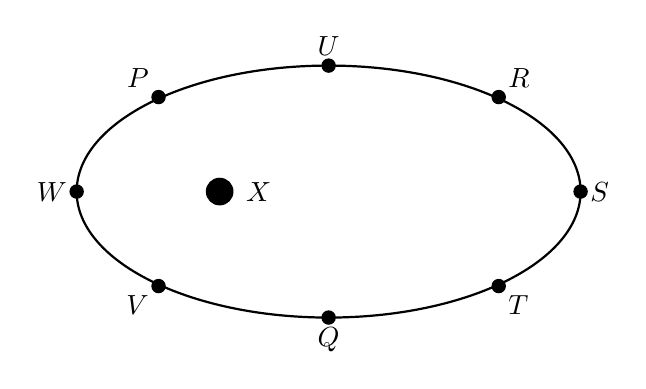
\begin{tikzpicture}[scale=0.8]
    %% orbit and center
    \draw[thick] (0,0) circle (4cm and 2cm);
    \draw[fill] (-1.73,0) circle (6pt) node[anchor=west,xshift=6pt] {$X$};
    %% Left and right
    \draw[fill] (-4,0) circle (3pt) node[anchor=east] {$W$};
    \draw[fill] (+4,0) circle (3pt) node[anchor=west] {$S$};
    %% top and bottom
    \draw[fill] (0,-2) circle (3pt) node[anchor=north] {$Q$};
    \draw[fill] (0,+2) circle (3pt) node[anchor=south] {$U$};
    %% diagonals (trial and error)
    \draw[fill] (-2.7,+1.5) circle (3pt) node[anchor=south east] {$P$};
    \draw[fill] (+2.7,+1.5) circle (3pt) node[anchor=south west] {$R$};
    \draw[fill] (+2.7,-1.5) circle (3pt) node[anchor=north west] {$T$};
    \draw[fill] (-2.7,-1.5) circle (3pt) node[anchor=north east] {$V$};
\end{tikzpicture}
}

\element{halliday-mc}{
\begin{question}{halliday-ch13-q40}
    A planet travels in an elliptical orbit about a star $X$ as shown. 
    \begin{center}
        \hallidayChThirteenQForty
    \end{center}
    The magnitude of the acceleration of the planet is:
    \begin{choices}
        \wrongchoice{greatest at point $Q$}
        \wrongchoice{greatest at point $S$}
        \wrongchoice{greatest at point $U$}
      \correctchoice{greatest at point $W$}
        \wrongchoice{the same at all points}
    \end{choices}
\end{question}
}

\element{halliday-mc}{
\begin{question}{halliday-ch13-q41}
    In planetary motion the line from the star to the planet sweeps out equal areas in equal times.
    This is a direct consequence of:
    \begin{choices}
        \wrongchoice{the conservation of energy}
        \wrongchoice{the conservation of momentum}
      \correctchoice{the conservation of angular momentum}
        \wrongchoice{the conservation of mass}
        \wrongchoice{none of the above}
    \end{choices}
\end{question}
}

\element{halliday-mc}{
\begin{question}{halliday-ch13-q42}
    The speed of a comet in an elliptical orbit about the Sun:
    \begin{choices}
      \correctchoice{decreases while it is receding from the Sun}
        \wrongchoice{is constant}
        \wrongchoice{is greatest when farthest from the Sun}
        \wrongchoice{varies sinusoidally with time}
        \wrongchoice{equals $L/(mr)$, where $L$ is its angular momentum, $m$ is its mass, and $r$ is its distance from the Sun}
    \end{choices}
\end{question}
}

\element{halliday-mc}{
\begin{question}{halliday-ch13-q43}
    A planet travels in an elliptical orbit about a star as shown. 
    \begin{center}
        \hallidayChThirteenQForty
    \end{center}
    At what pair of points is the speed of the planet the same?
    \begin{multicols}{2}
    \begin{choices}
        \wrongchoice{$W$ and $S$}
        \wrongchoice{$P$ and $T$}
        \wrongchoice{$P$ and $R$}
      \correctchoice{$Q$ and $U$}
        \wrongchoice{$V$ and $R$}
    \end{choices}
    \end{multicols}
\end{question}
}

\element{halliday-mc}{
\begin{question}{halliday-ch13-q44}
    Planet 1 and planet 2 are both in circular orbits around the same central star. 
    The orbit of planet 2 has a radius that is much larger than the radius of the orbit of planet 1. 
    This means that:
    \begin{choices}
        \wrongchoice{the period of planet 1 is greater than the period of planet 2 and the speed of planet 1 is greater than the speed of planet 2}
        \wrongchoice{the period of planet 1 is greater than the period of planet 2 and the speed of planet 1 is less than the speed of planet 2}
        \wrongchoice{the period of planet 1 is less than the period of planet 2 and the speed of planet 1 is less than the speed of planet 2}
      \correctchoice{the period of planet 1 is less than the period of planet 2 and the speed of planet 1 is greater than the speed of planet 2}
        \wrongchoice{the planets have the same speed and the same period}
    \end{choices}
\end{question}
}

\element{halliday-mc}{
\begin{question}{halliday-ch13-q45}
    For a planet in orbit around a star the perihelion distance is $r_p$ ad its speed at perihelion is $v_p$.
    The aphelion distance is $r_a$ and its speed at aphelion is $v_a$.
    Which of the following is true?
    \begin{multicols}{2}
    \begin{choices}
        \wrongchoice{$v_a               = v_p$}
        \wrongchoice{$\dfrac{v_a}{r_a}  = \dfrac{v_p }{r_p}$}
      \correctchoice{$v_a r_a           = v_p r_p$}
        \wrongchoice{$\dfrac{v_a}{r_a^2}= \dfrac{v_p }{r_p^2}$}
        \wrongchoice{$v_a r_a^2         = v_p r_p^2$}
    \end{choices}
    \end{multicols}
\end{question}
}

\element{halliday-mc}{
\begin{question}{halliday-ch13-q46}
    A planet is in circular orbit around the Sun. 
    Its distance from the Sun is four times the average distance of Earth from the Sun. 
    The period of this planet,
        in Earth years, is:
    \begin{multicols}{3}
    \begin{choices}
        \wrongchoice{\num{4}}
      \correctchoice{\num{8}}
        \wrongchoice{\num{16}}
        \wrongchoice{\num{64}}
        \wrongchoice{\num{2.52}}
    \end{choices}
    \end{multicols}
\end{question}
}

\element{halliday-mc}{
\begin{question}{halliday-ch13-q47}
    Two planets are orbiting a star in a distant galaxy. 
    The first has a semimajor axis of \SI{150e6}{\kilo\meter},
        an eccentricity of \num{0.20}, and a period of \num{1.0} Earth years. 
    The second has a semimajor axis of \SI{250e6}{\kilo\meter},
        an eccentricity of \num{0.30}, and a period of:
    \begin{multicols}{2}
    \begin{choices}
        \wrongchoice{\num{0.46} Earth years}
        \wrongchoice{\num{0.57} Earth years}
        \wrongchoice{\num{1.4} Earth years}
        \wrongchoice{\num{1.8} Earth years}
      \correctchoice{\num{2.2} Earth years}
    \end{choices}
    \end{multicols}
\end{question}
}

\element{halliday-mc}{
\begin{question}{halliday-ch13-q48}
    A small satellite is in elliptical orbit around Earth as shown. 
    \begin{center}
    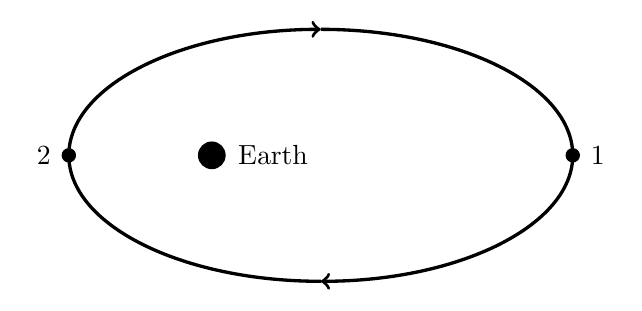
\begin{tikzpicture}[scale=0.8]
        %% orbit
        \draw[very thick,->] (0,-2) arc (270:90:4cm and 2cm);
        \draw[very thick,->] (0,+2) arc (90:-90:4cm and 2cm);
        %% labels
        \draw[fill] (-4,0) circle (3pt) node[anchor=east,xshift=-3pt] {2};
        \draw[fill] (+4,0) circle (3pt) node[anchor=west,xshift=+3pt] {1};
        %% earth
        %\draw[fill] (-1.12,0) circle (6pt)  node[anchor=west,xshift=6pt] {Earth};
        \draw[fill] (-1.73,0) circle (6pt)  node[anchor=west,xshift=6pt] {Earth};
    \end{tikzpicture}
    \end{center}
    If $L$ denotes the magnitude of its angular momentum and $K$ denotes kinetic energy:
    \begin{choices}
        \wrongchoice{$L_2 > L_1$ and $K_2 > K_1$}
        \wrongchoice{$L_2 > L_1$ and $K_2 = K_1$}
        \wrongchoice{$L_2 = L_1$ and $K_2 = K_1$}
        \wrongchoice{$L_2 < L_1$ and $K_2 = K_1$}
      \correctchoice{$L_2 = L_1$ and $K_2 > K_1$}
    \end{choices}
\end{question}
}

\element{halliday-mc}{
\begin{question}{halliday-ch13-q49}
    Assume that Earth is in circular orbit around the Sun with kinetic energy $K$ and potential energy $U$,
        taken to be zero for infinite separation. 
    Then, the relationship between $K$ and $U$:
    \begin{multicols}{2}
    \begin{choices}
        \wrongchoice{is $K = U$}
        \wrongchoice{is $K = -U$}
        \wrongchoice{is $K = \dfrac{U}{2}$}
      \correctchoice{is $K = -\dfrac{U}{2}$}
        \wrongchoice{depends on the radius of the orbit}
    \end{choices}
    \end{multicols}
\end{question}
}

\element{halliday-mc}{
\begin{question}{halliday-ch13-q50}
    An artificial Earth satellite is moved from a circular orbit with radius $R$ to a circular orbit with radius $2R$. 
    During this move:
    \begin{choices}
        \wrongchoice{the gravitational force does positive work, the kinetic energy of the satellite increases, and the potential energy of the Earth-satellite system increases}
        \wrongchoice{the gravitational force does positive work, the kinetic energy of the satellite increases, and the potential energy of the Earth-satellite system decreases}
        \wrongchoice{the gravitational force does positive work, the kinetic energy of the satellite decreases, and the potential energy of the Earth-satellite system increases}
        \wrongchoice{the gravitational force does negative work, the kinetic energy of the satellite increases, and the potential energy of the Earth-satellite system decreases}
      \correctchoice{the gravitational force does negative work, the kinetic energy of the satellite decreases, and the potential energy of the Earth-satellite system increases}
    \end{choices}
\end{question}
}

\element{halliday-mc}{
\begin{question}{halliday-ch13-q51}
    An artificial satellite of Earth nears the end of its life due to air resistance. 
    While still in orbit:
    \begin{choices}
      \correctchoice{it moves faster as the orbit lowers}
        \wrongchoice{it moves slower as the orbit lowers}
        \wrongchoice{it slowly spirals away from Earth}
        \wrongchoice{it moves slower in the same orbit but with a decreasing period}
        \wrongchoice{it moves faster in the same orbit but with an increasing period}
    \end{choices}
\end{question}
}

\element{halliday-mc}{
\begin{question}{halliday-ch13-q52}
    A spaceship is returning to Earth with its engine turned off. 
    Consider only the gravitational field of Earth and let $M$ be the mass of Earth,
        $m$ be the mass of the spaceship,
        and $R$ be the distance from the center of Earth. 
    In moving from position 1 to position 2 the kinetic energy of the spaceship increases by:
    \begin{choices}
        \wrongchoice{$GMm\left[\dfrac{1}{R_2^2}-\dfrac{1}{F_1^2}\right] \dfrac{GHm}{R_2}$}
        \wrongchoice{$GMm\left[\dfrac{1}{R_2^2}+\dfrac{1}{F_1^2}\right]$}
        \wrongchoice{$GMm\dfrac{R_1-R_2}{R_1^2}$}
      \correctchoice{$GMm\dfrac{R_1-R_2}{R_1 R_2}$}
        \wrongchoice{$GMm\dfrac{R_1-R_2}{R_1^2 R_2^2}$}
    \end{choices}
\end{question}
}

\element{halliday-mc}{
\begin{question}{halliday-ch13-q53}
    Given the perihelion distance, aphelion distance,
        and speed at perihelion of a planet,
        which of the following \emph{cannot} be calculated?
    \begin{choices}
        \wrongchoice{The mass of the star}
      \correctchoice{The mass of the planet}
        \wrongchoice{The speed of the planet at aphelion}
        \wrongchoice{The period of orbit}
        \wrongchoice{The semimajor axis of the orbit}
    \end{choices}
\end{question}
}

\element{halliday-mc}{
\begin{question}{halliday-ch13-q54}
    The orbit of a certain satellite has a semimajor axis of \SI{1.5e7}{\meter} and an eccentricity of \num{0.20}.
    Its perigee (minimum distance) and apogee (maximum distance) are respectively:
    \begin{choices}
      \correctchoice{\SI{1.2e7}{\meter}, \SI{1.8e7}{\meter}}
        \wrongchoice{\SI{3.0e6}{\meter}, \SI{1.2e7}{\meter}}
        \wrongchoice{\SI{9.6e6}{\meter}, \SI{1.0e7}{\meter}}
        \wrongchoice{\SI{1.0e7}{\meter}, \SI{1.2e7}{\meter}}
        \wrongchoice{\SI{9.6e6}{\meter}, \SI{1.8e7}{\meter}}
    \end{choices}
\end{question}
}

\element{halliday-mc}{
\begin{question}{halliday-ch13-q55}
    A planet in another solar system orbits a star with a mass of \SI{4.0e30}{\kilo\gram}.
    At one point in its orbit it is \SI{250e6}{\kilo\meter} from the star and is moving at \SI{35}{\kilo\meter\per\second}.
    Take the universal gravitational constant to be \SI{6.67e-11}{\meter\squared\per\second\squared\per\kilo\gram}
        and calculate the semimajor axis of the planet's orbit.
    The result is:
    \begin{multicols}{2}
    \begin{choices}
        \wrongchoice{\SI{79e6}{\kilo\meter}}
        \wrongchoice{\SI{160e6}{\kilo\meter}}
      \correctchoice{\SI{290e6}{\kilo\meter}}
        \wrongchoice{\SI{320e6}{\kilo\meter}}
        \wrongchoice{\SI{590e6}{\kilo\meter}}
    \end{choices}
    \end{multicols}
\end{question}
}


\endinput


